% Intended LaTeX compiler: xelatex
\documentclass[a4paper, 12pt]{article}
\usepackage{graphicx}
\usepackage{longtable}
\usepackage{wrapfig}
\usepackage{rotating}
\usepackage[normalem]{ulem}
\usepackage{amsmath}
\usepackage{amssymb}
\usepackage{capt-of}
\usepackage{hyperref}
\usepackage[danish]{babel}
\usepackage{mathtools}
\usepackage[margin=3.0cm]{geometry}
\hypersetup{colorlinks, linkcolor=black, urlcolor=blue}
\setlength{\parindent}{0em}
\parskip 1.5ex
\author{Jacob Debel}
\date{Fysik C \& B}
\title{Lys og bølger\\\medskip
\large Konstruktion - Det optiske gitter}
\hypersetup{
 pdfauthor={Jacob Debel},
 pdftitle={Lys og bølger},
 pdfkeywords={},
 pdfsubject={},
 pdfcreator={Emacs 29.4 (Org mode 9.6.15)}, 
 pdflang={Danish}}
\begin{document}

\maketitle
På de nedenstående figurer skal I tegne/indsætte de følgende fysiske størrelser:

\(\lambda\), \(2 \lambda\), \(d\), \(\phi_1\), \(\phi_2\), normal, plane bølger, ny bølgefront, udbredelsesretning.

Størrelserne må gerne bruges flere gange, hvis det passer ind.

\begin{center}
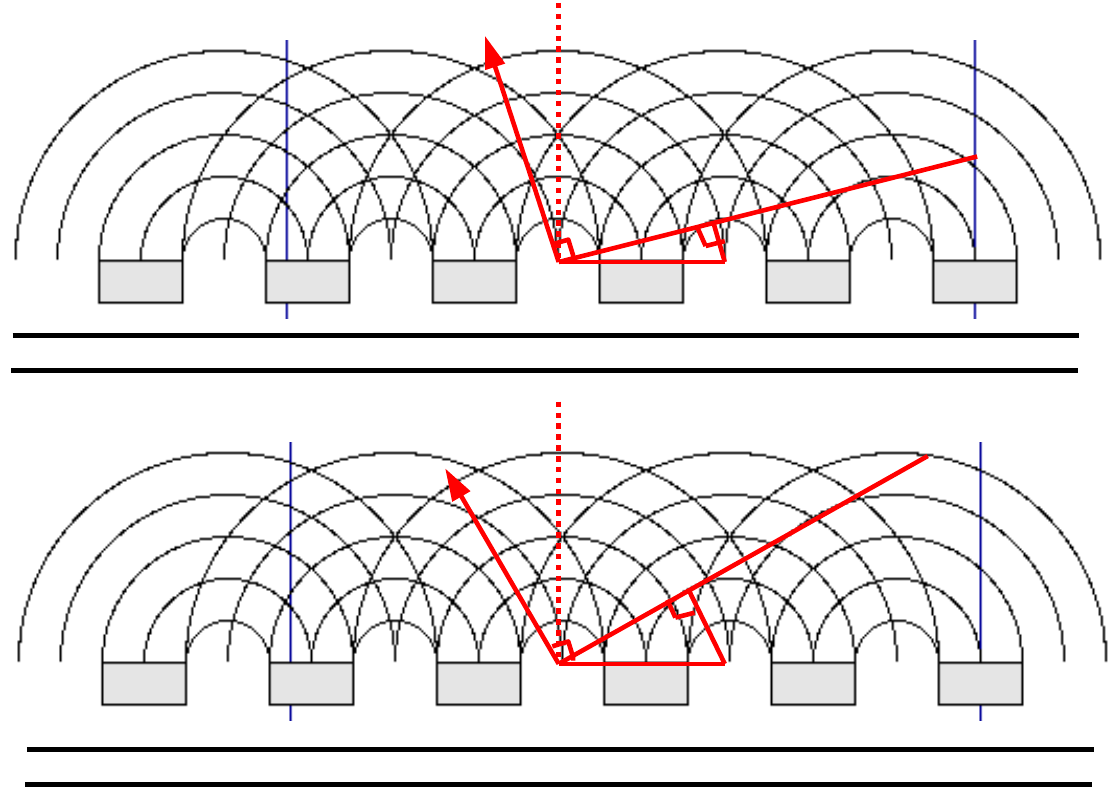
\includegraphics[width=.9\linewidth]{./img/gitterudledning.png}
\end{center}

\begin{itemize}
\item På baggrund af ovenstående skitser og de førnævnte fysiske størrelser \textbf{skal I nu udlede gitterligningen} med en så kort og præcis formulering, som I magter. Husk at bruge de rette fagudtryk.

\item \textbf{I må gerne bruge jeres noter, men ikke bogen.}

\item \textbf{Jeres skitser med indsatte størrelser og jeres udledninger skal afleveres.}
\end{itemize}
\end{document}
